For all parts of this question I have assumed $T = 300 \textrm{ K}$ and have used values appropriate for silicon.
\subsection*{a)}
	\begin{figure}[htbp!]
		%	\centering
		\flushright
		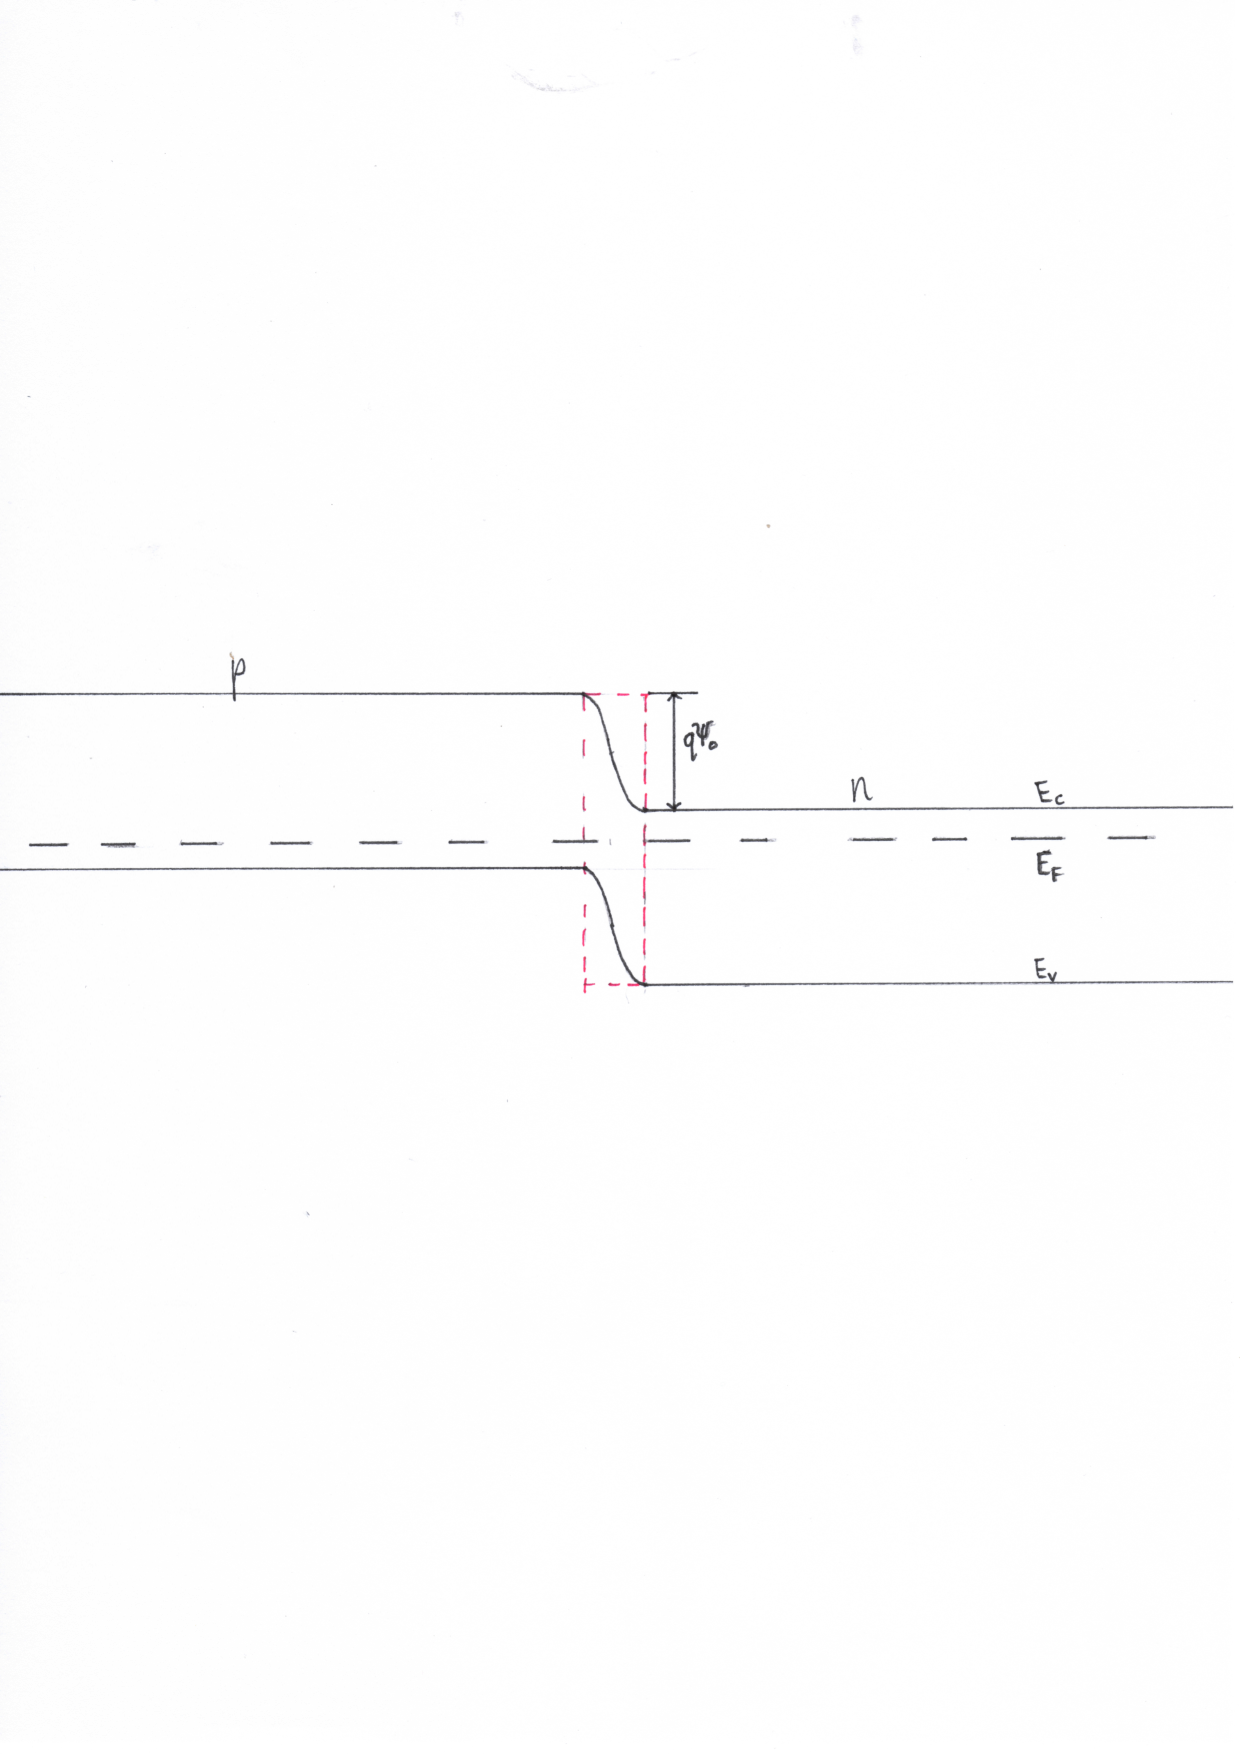
\includegraphics[trim={3.5cm 12.5cm 2.5cm 11cm},clip]{./img/2a}
		\caption{Energy diagram of a pn junction.}
	\end{figure}
	\[
	\begin{aligned}
		q \psi_0 &= E_C(p) - E_C(n) \\
			   &= (E_F + E_G - E_1) - (E_F + E_2) \\
			   &= E_G - E_1 - E_2 \\
			   &= 1.12 \textrm{ eV} - k T \ln \left( \frac{N_V N_C}{N_A N_D} \right) \\
			\psi_0  &=	1.12 \textrm{ V} - 0.147 \textrm{ V} \\
			   &= 0.973 \textrm{ V}	   
	\end{aligned}
	\]
\subsection*{b)}
	Under forward-bias, electrons are injected into the n-doped regions, and positive charges, or holes, 
	will be injected into the p-doped region. An electron injected into the n-doped region will feel an electric attraction due to the positive-space charge region and so will accelerate, and be swept into the p-doped region, as a drift current. Once in the p-region, it can readily recombine with a hole. Once carriers have recombined, we have reached our initial conditions, and the process will repeat. Due to the recombination current, more current will be drawn from the applied voltage source. A similar explanation can be applied to the holes injected into the p-doped region, being swept into the n-doped region. Therefore, the minority carriers define the large portion of the total diode current.
\subsection*{c)}
	
